\documentclass[12pt, titlepage]{article}

\usepackage[ngerman]{babel}
\usepackage{color}
\usepackage[a4paper,lmargin={4cm},rmargin={2cm},
tmargin={2.5cm},bmargin = {2.5cm}]{geometry}
\usepackage{amssymb}
\usepackage{amsthm}
\usepackage{amsmath}
\usepackage{graphicx}
\usepackage[utf8]{inputenc}
\usepackage{hyperref}
\usepackage{listings}

\definecolor{mygreen}{rgb}{0,0.6,0}
\definecolor{mygray}{rgb}{0.50,0,0.5}
\definecolor{mymauve}{rgb}{0.58,0,0.82}

\setcounter{MaxMatrixCols}{20}

\lstset{
	breaklines=true,
	frame=single,
	numbers=left,
	stepnumber=5,
	language=C++,
	keywordstyle=\color{blue},
	commentstyle=\color{mygreen},
	backgroundcolor=\color{white},
	numberstyle=\color{mygray},
	stringstyle=\color{mymauve},
	tabsize=2
}

\begin{document}
\begin{titlepage}
	\title{Prüfungsvorleistung Codierungs-Theorie}
	\author{David Tarnow, Michael Narkus, Armel Siewe, Lukas Köhler}
	\maketitle
\end{titlepage}
	
\tableofcontents

\newpage









\section{Einführung}
Einführung in die Thematik. Aufbau der Applikation, Imports (Gurobi, armadillo und co)
\subsection{Verwendung von C++}
Als Programmiersprache wurde in diesem Projekt C++ verwendet. Die entscheidenden Gründe für C++ waren zum einen die hohe Performance sowie die existierenden Bibliotheken (z.B. Armadillo) und Schnittstellen für die Nutzung von Gurobi.  
\subsection{Armadillo}
\href{http://arma.sourceforge.net/}{Armadillo} ist eine C++-Bibliothek, welche Funktionen und Klassen zur linearen Algebra bereitstellt. Angelehnt an MatLab werden hier Klassen für Vektoren, Matrizen und Kuben bereitgestellt.
Im Rahmen dieses Projektes wurde Armadillo in der neusten stabilen Version (8.500.1) verwendet. \\
\subsection{Gurobi}
Mit dem Gurobi Solver wurde im Rahmen dieser Praktikumsaufgabe eine externe Software genutzt um die Optimierungsprobleme zu lösen. Eine Schnittstelle zur Ansteuerung des Gurobi-Solvers in der Version 8.5.0 wird hier vom Hersteller bereitgestellt. 
\subsection{LAPACK}
Als Abhängigkeit von Armadillo wurde außerdem LAPACK genutzt. Um die komplexeren Berechnungen, welche mit Armadillo durchgeführt werden können, zu beschleunigen, wird unter Windows OpenBLAS (oder Intel MK) benötigt. Die Bibliothek LAPACK stellt hierfür ebenfalls Komponenten bereit.














\section{Konstruktion der Matrix A}
Zunächst werden die linear unabhängigen Vektoren für gegebene Werte q und k (nur Primzahlen) berechnet.
Daraus ergeben sich insgesamt q$^k$ -1 Vektoren, die in $\dfrac{q^{k}-1}{q-1}$ Klassen eingeteilt werden können.
Dabei besitzt jede Klasse genau q - 1 Vielfache.
Die Berechnung der linear unabhängigen Vektoren erfolgt im gegebenen Programm rekursiv.

\newpage
Es wird im folgenden der Fall für q = 3 und k = 3 betrachtet.
Dabei ergeben sich folgende linear unabhängigen Vektoren:
\begin{description}
\item r0 = (0 0 1)$^T$
\item r1 = (0 1 0)$^T$
\item r2 = (0 1 1)$^T$
\item r3 = (0 1 2)$^T$
\item r4 = (1 0 0)$^T$
\item r5 = (1 0 1)$^T$
\item r6 = (1 0 2)$^T$
\item r7 = (1 1 0)$^T$
\item r8 = (1 1 1)$^T$
\item r9 = (1 1 2)$^T$
\item r10 = (1 2 0)$^T$
\item r11 = (1 2 1)$^T$
\item r12 = (1 2 2)$^T$
\end{description}

Im Anschluss wird die Matrix A der Form $A_{k,q}$ konstruiert.
Dies geschieht innerhalb von geschachtelten for- Schleifen, die jeweils das Skalarprodukt von zwei Repräsentanten berechnet.
Das Ergebnis wird modulo \textit{q} genommen.
Sofern das Ergebnis gleich Null ist, wird in der Matrix die entsprechende Stelle auf 1 gesetzt, andernfalls auf 0.
Bei der beispielhaften Eingabe erhalten wir folgende Werte:

\begin{center}
\item
$A_{3,3}$ = 		
$
\begin{pmatrix}
	0 & 1 & 0 & 0 & 1 & 0 & 0 & 1 & 0 & 0 & 1 & 0 & 0 \\
	1 & 0 & 0 & 0 & 1 & 1 & 1 & 0 & 0 & 0 & 0 & 0 & 0 \\
	0 & 0 & 0 & 1 & 1 & 0 & 0 & 0 & 0 & 1 & 0 & 1 & 0 \\
	0 & 0 & 1 & 0 & 1 & 0 & 0 & 0 & 1 & 0 & 0 & 0 & 1 \\
	1 & 1 & 1 & 1 & 0 & 0 & 0 & 0 & 0 & 0 & 0 & 0 & 0 \\
	0 & 1 & 0 & 0 & 0 & 0 & 1 & 0 & 0 & 1 & 0 & 0 & 1 \\
	0 & 1 & 0 & 0 & 0 & 1 & 0 & 0 & 1 & 0 & 0 & 1 & 0 \\
	1 & 0 & 0 & 0 & 0 & 0 & 0 & 0 & 0 & 0 & 1 & 1 & 1 \\
	0 & 0 & 0 & 1 & 0 & 0 & 1 & 0 & 1 & 0 & 1 & 0 & 0 \\
	0 & 0 & 1 & 0 & 0 & 1 & 0 & 0 & 0 & 1 & 1 & 0 & 0 \\
	1 & 0 & 0 & 0 & 0 & 0 & 0 & 1 & 1 & 1 & 0 & 0 & 0 \\
	0 & 0 & 1 & 0 & 0 & 0 & 1 & 1 & 0 & 0 & 0 & 1 & 0 \\
	0 & 0 & 0 & 1 & 0 & 1 & 0 & 1 & 0 & 0 & 0 & 0 & 1 \\
\end{pmatrix}
$
\end{center}

Es wurden ebenfalls deutlich höhere Werte für k und q getestet, die jedoch den Rahmen dieser Ausarbeitung sprengen würden.










\section{Optimierungsproblem}

Um das wachsende Optimierungsproblem \textit{max\{$<$1,x$>$ | $A_{k,q}$x $\leq$ b\}}  zu lösen, wird die Software GUROBI genutzt.
Diese optimiert die Werte für den gesuchten Vektor x bei einem eingegeben Vektor c von
\begin{center}
c = (1 1 1 1 1 1 1 1 1 1 1 1 1)$^T$

x = (0 0 0 0 1 1 1 1 1 1 1 1 1)$^T$
\end{center}









	
\section{Codetabellen}

Für den nächsten Schritt betrachten wir den Fall für q = 7 und k = 3.
Dabei ergibt sich schon eine deutlich größere Matrix A, sowie der Vektor x wie folgt:
\begin{center}
x = (1 0 0 0 0 0 1 0 0 0 0 1 0 0 0 0 0 0 1 0 0 1 1 0 0 0 0 1 0 1 0 0 0 0 1 0 0 0 0 0 0 1 1 0 0 1 0 0 0 1 0 0 1 1 0 0 0)$^T$
\end{center}
Die dazugehörige Generatormatrix G berechnet sich dabei anhand des Vektors x, der angibt, welche Repräsentanten an welche Stelle eingefügt werden sollen.
Im gegeben Beispiel ergibt sich:
\begin{center}
\item
G = 	
$
\begin{pmatrix}
	0 & 0 & 1 & 1 & 1 & 1 & 1 & 1 & 1 & 1 & 1 & 1 & 1 & 1 & 1 \\
	0 & 1 & 0 & 1 & 1 & 2 & 2 & 3 & 3 & 4 & 4 & 5 & 5 & 6 & 6 \\
	1 & 5 & 3 & 3 & 6 & 0 & 5 & 0 & 5 & 5 & 6 & 2 & 6 & 2 & 3 \\
\end{pmatrix}
$
\end{center}

Der daraus resultierende Code ist ein [15, 3, 12]$_q$ Code.
Um die gegebene Minimaldistanz d zu verifizieren wird die Hamming-Distanz manuell berechnet.
Dazu werden zunächst alle möglichen Nachrichtenwörter für die gegebenen q und k generiert (mit Ausnahme des Nullwortes) und mit der Generatormatrix G kodiert.
Anschließend wird von jedem Codewort zu jedem anderen Codewort (mit Ausnahme zu sich selbst) die Hamming-Distanz berechnet und anschließend der Minimalwert zurückgeliefert.
In unserem Beispiel ergibt sich dabei: \\
12 = calculated distance, 12 = should be the distance \\







\section{Zyklenerkennung}

Da mit steigendem q und k ebenfalls die Matrix $A_{k,q}$ anwächst wird es für GUROBI zunehmend aufwändiger eine Lösung für den Vektor x zu finden.
Um die eingegebene Matrix zu reduzieren wird daher eine Erzeugermatrix \textit{e} der Größe k x k gesucht, die anschließend auf die einzelnen Repräsentanten angewandt wird.
Sofern eine Konvertierung in eine andere Gruppe möglich ist wird eine entsprechende Queue angelegt.
In dem Fall, dass sowohl Anfangs- als auch Endpunkt das gleiche Element sind kann ein Zyklus festgehalten werden.
Als Beispiel für q = 7, k = 3 und b = 3 kann die Matrix $A_{k,q}$ der Größe 57 x 57 auf eine 13 x 13 Matrix reduziert werden.
\begin{center}
\item
e = 	
$
\begin{pmatrix}
	6 & 0 & 0 \\
	6 & 5 & 4 \\
	6 & 0 & 4 \\
\end{pmatrix}
$
\end{center}



\newpage
Daraus ergeben sich folgende Gruppen für die Spalten:

\begin{description}
\item S([r0]) = {[r0], [r2], [r3], [r4], [r5], [r7]}
\item S([r1]) = {[r1]}
\item S([r6]) = {[r6]}
\item S([r8]) = {[r8], [r10], [r16], [r42], [r54], [r55]}
\item S([r9]) = {[r9], [r14], [r29], [r40], [r45], [r48]}
\item S([r11]) = {[r11], [r25], [r32]}
\item S([r12]) = {[r12], [r17], [r22], [r34], [r44], [r56]}
\item S([r13]) = {[r13], [r19], [r21], [r23], [r24], [r36]}
\item S([r15]) = {[r15], [r20], [r30], [r33], [r38], [r49]}
\item S([r18]) = {[r18], [r46], [r53]}
\item S([r26]) = {[r26], [r31], [r35], [r41], [r50], [r51]}
\item S([r27]) = {[r27], [r28], [r37], [r43], [r47], [r52]}
\item S([r39]) = {[r39]}
\end{description}

Sowie für die Reihen (mit transponiertem e$^T$)

\begin{description}
\item S$^T$([r0]) = {[r0], [r9], [r11], [r12], [r13], [r14]}
\item S$^T$([r1]) = {[r1], [r7], [r24], [r25], [r35], [r44]}
\item S$^T$([r2]) = {[r2], [r18], [r26], [r42], [r43], [r51]}
\item S$^T$([r3]) = {[r3], [r4], [r15], [r20], [r32], [r39]}
\item S$^T$([r5]) = {[r5], [r38], [r53]}
\item S$^T$([r6]) = {[r6], [r33], [r46], [r48], [r50], [r54]}
\item S$^T$([r8]) = {[r8]}
\item S$^T$([r10]) = {[r10]}
\item S$^T$([r16]) = {[r16], [r21], [r22], [r31], [r52], [r55]}
\item S$^T$([r17]) = {[r17], [r29], [r40], [r41], [r45], [r47]}
\item S$^T$([r19]) = {[r19], [r23], [r49]}
\item S$^T$([r27]) = {[r27], [r28], [r30], [r36], [r37], [r56]}
\item S$^T$([r34]) = {[r34]}
\end{description}



\newpage
Im Anschluss daran werden in den Spalten die jeweiligen Gruppen zusammenaddiert bzw. in den Reihen die überflüssigen Reihen entfernt, sodass sich die verkleinerte Matrix

\begin{center}
\item
$A_{3,7}$ = 		
$
\begin{pmatrix}
	0 & 1 & 0 & 1 & 1 & 0 & 1 & 1 & 1 & 0 & 1 & 1 & 0 \\
	1 & 0 & 0 & 2 & 2 & 1 & 1 & 1 & 0 & 0 & 0 & 0 & 0 \\
	1 & 0 & 0 & 1 & 1 & 0 & 0 & 1 & 1 & 0 & 1  &1 & 1 \\
	1 & 0 & 0 & 2 & 0 & 0 & 1 & 0 & 0 & 1 & 2 & 1 & 0 \\
	0 & 0 & 1 & 2 & 0 & 1 & 0 & 0 & 2 & 0 & 0 & 2 & 0 \\
	1 & 0 & 0 & 1 & 0 & 0 & 1 & 2 & 2 & 1 & 0 & 0 & 0 \\
	6 & 1 & 1 & 0 & 0 & 0 & 0 & 0 & 0 & 0 & 0 & 0 & 0 \\
	0 & 1 & 0 & 0 & 0 & 3 & 0 & 0 & 0 & 3 & 0 & 0 & 1 \\
	1 & 0 & 0 & 0 & 1 & 1 & 1 & 0 & 2 & 0 & 2 & 0 & 0 \\
	1 & 0 & 0 & 0 & 0 & 1 & 1 & 2 & 0 & 0 & 1 & 2 & 0 \\
	0 & 0 & 1 & 0 & 2 & 0 & 0 & 2 & 0 & 1 & 2 & 0 & 0 \\
	1 & 0 & 0 & 0 & 2 & 0 & 1 & 0 & 1 & 1 & 0 & 2 & 0 \\
	0 & 0 & 1 & 0 & 0 & 0 & 6 & 0 & 0 & 0 & 0 & 0 & 1 \\
\end{pmatrix}
$
\end{center}

mit den daraus resultierenden Vektoren

\begin{center}
c = (6 1 1 6 6 3 6 6 6 3 6 6 1)$^T$

x = (0 1 1 0 0 0 0 0 0 0 1 1 1)$^T$
\end{center}

Insgesamt ergibt sich dadurch ein [15, 3, 12]$_7$ Code.









\section{Generierung des Erzeugers}

Schließlich ist die Herausforderung einen Erzeuger e zu finden, der die Matrix A soweit vereinfacht, sodass GUROBI das Optimierungsproblem in einer angemessenen Zeit lösen kann.
Bei den Tests ist aufgefallen, dass vergleichsweise kleine Matrizen A sich ebenfalls auf die Länge des Nachrichtenwortes \textit{n}.
Diese wird mit zunehmender Größe der Matrix A ebenfalls größer, sodass ein Codewort mit der Länge k ebenfalls in mehr Bits kodiert werden kann.

Um möglichst große \textit{n} zu erzeugen muss nun der Erzeuger e so gewählt werden, dass er zwar die Matrix A in der Größe reduziert jedoch nur so weit wie nötig, sodass das Optimierungsproblem in akzeptabler Zeit lösbar ist bzw. überhaupt eine Lösung gefunden werden kann.





\newpage
\begin{figure}
	\centering
	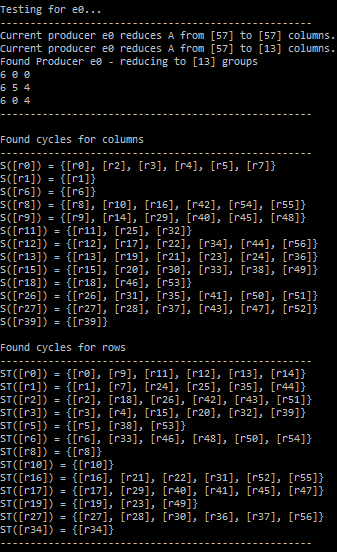
\includegraphics[width=1.0\textwidth]{screenshot/grouping.png}
 \end{figure}


\begin{figure}
	\centering
	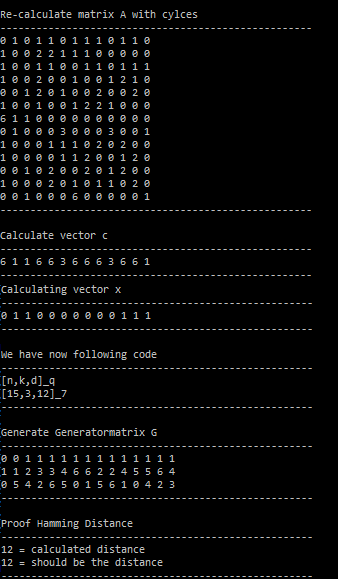
\includegraphics[width=1.0\textwidth]{screenshot/result.png}
 \end{figure}


















	
\end{document}